%%%%%%%%%%%%%%%%%%%%%%%%%%%%%%%%%%%%%%%%%
% Template
% LaTeX Template
% Version 1.0 (December 8 2014)
%
% This template has been downloaded from:
% http://www.LaTeXTemplates.com
%
% Original author:
% Brandon Fryslie
% With extensive modifications by:
% Vel (vel@latextemplates.com)
%
% License:
% CC BY-NC-SA 3.0 (http://creativecommons.org/licenses/by-nc-sa/3.0/)
%
% Authors:
% Sabbir Ahmed
% 
%%%%%%%%%%%%%%%%%%%%%%%%%%%%%%%%%%%%%%%%%

\documentclass[paper=usletter, fontsize=12pt]{article}
%%%%%%%%%%%%%%%%%%%%%%%%%%%%%%%%%%%%%%%%%
% Contract Structural Definitions File Version 1.0 (December 8 2014)
%
% Created by: Vel (vel@latextemplates.com)
% 
% This file has been downloaded from: http://www.LaTeXTemplates.com
%
% License: CC BY-NC-SA 3.0 (http://creativecommons.org/licenses/by-nc-sa/3.0/)
%
%%%%%%%%%%%%%%%%%%%%%%%%%%%%%%%%%%%%%%%%%

\usepackage{geometry} % Required to modify the page layout
\usepackage{multicol}
\usepackage{amsmath}
\usepackage{amssymb}

\usepackage[pdftex]{graphicx}
\usepackage{wrapfig}
\usepackage[font=scriptsize, labelfont=bf]{caption}
\usepackage[utf8]{inputenc} % Required for including letters with accents
\usepackage[T1]{fontenc} % Use 8-bit encoding that has 256 glyphs

\usepackage{avant} % Use the Avantgarde font for headings
\usepackage{courier}
\usepackage{xparse}
\usepackage{xcolor}
\usepackage{listings}  % for code verbatim and console outputs

\setlength{\textwidth}{16cm} % Width of the text on the page
\setlength{\textheight}{23cm} % Height of the text on the page
\setlength{\oddsidemargin}{0cm} % Width of the margin - negative to move text left, positive to move it right
\setlength{\topmargin}{-1.25cm} % Reduce the top margin

\setlength{\parindent}{0mm} % Don't indent paragraphs
\setlength{\parskip}{2.5mm} % Whitespace between paragraphs
\renewcommand{\baselinestretch}{1.5}

\definecolor{green}{rgb}{0.18, 0.55, 0.34}

\graphicspath{ {figures/} }
\captionsetup[table]{skip=10pt}

\lstset{language=C, keywordstyle={\bfseries \color{black}}}

% defines algorithm counter for chapter-level
\newcounter{nalg}[section]

%defines appearance of the algorithm counter
\renewcommand{\thenalg}{\thesection .\arabic{nalg}}

% defines a new caption label as Algorithm x.y
\DeclareCaptionLabelFormat{algocaption}{Algorithm \thenalg}

% defines the algorithm listing environment
\lstnewenvironment{pseudocode}[1][] {
    \refstepcounter{nalg}  % increments algorithm number
    \captionsetup{font=normalsize, labelformat=algocaption, labelsep=colon}
    \lstset{
        breaklines=true,
        mathescape=true,
        numbers=left,
        numberstyle=\scriptsize,
        basicstyle=\footnotesize\ttfamily,
        keywordstyle=\color{black}\bfseries,
        keywords={input, output, return, parallel, function, for, to, in, if,
        else, foreach, while, and, or, new, print},
        xleftmargin=.04\textwidth,
        #1
    }
}{}

\renewcommand{\familydefault}{\sfdefault}  % default font for entire document
 % specifies the document layout and style

\begin{document}

    \documentinfo{\textbf{Homework 3: Light the Candles}}{\today}{Sabbir Ahmed}
    \vspace{-0.1in}

    \section{Background}
    For this assignment, a game was created to be played on the development board. The goal of the game is for the player to light all the candles, represented by the 8 LEDs on the board just above the switches, while they are being pseudo-randomly turned off.
    
    The game starts off with the player pressing the RESET button (a.k.a. BTN\_SOUTH) just below the rotatory knob.

    The player is placed initially at a position 0.

    The player may light the candles by jumping on them. This is done using the BTN\_NORTH button on the board just above the rotary knob. A player may jump at the current position by setting the switches to zero and pressing BTN\_NORTH. Any desired horizontal movement in the jump to another position is provide by the four switches which indicate a value from 7 to -8, in binary two's compliment.

    Once a candle is lit, the player may jump again jump on the same location (using 0) or to another location using the delta provide by the switches.

    However, the candles that were lit will continually go out at random and must be relit. To be specific, a candle may at random go out at the same time the player jumps. Secondly, note that there is no direct indicator to where the player is; so it is up to the player to keep track.

    \section{Implementation}
    Three discrete modules were used to implement the game: \inlsnip{igniter}, \inlsnip{extinguisher} and \inlsnip{candle_controller}. These submodules were connected and debounced using a top level module that may be visualized with the schematic diagram configured as a block diagram in Figure \ref{fig:schematic}.

    \begin{figure}[ht]
        \begin{center}
            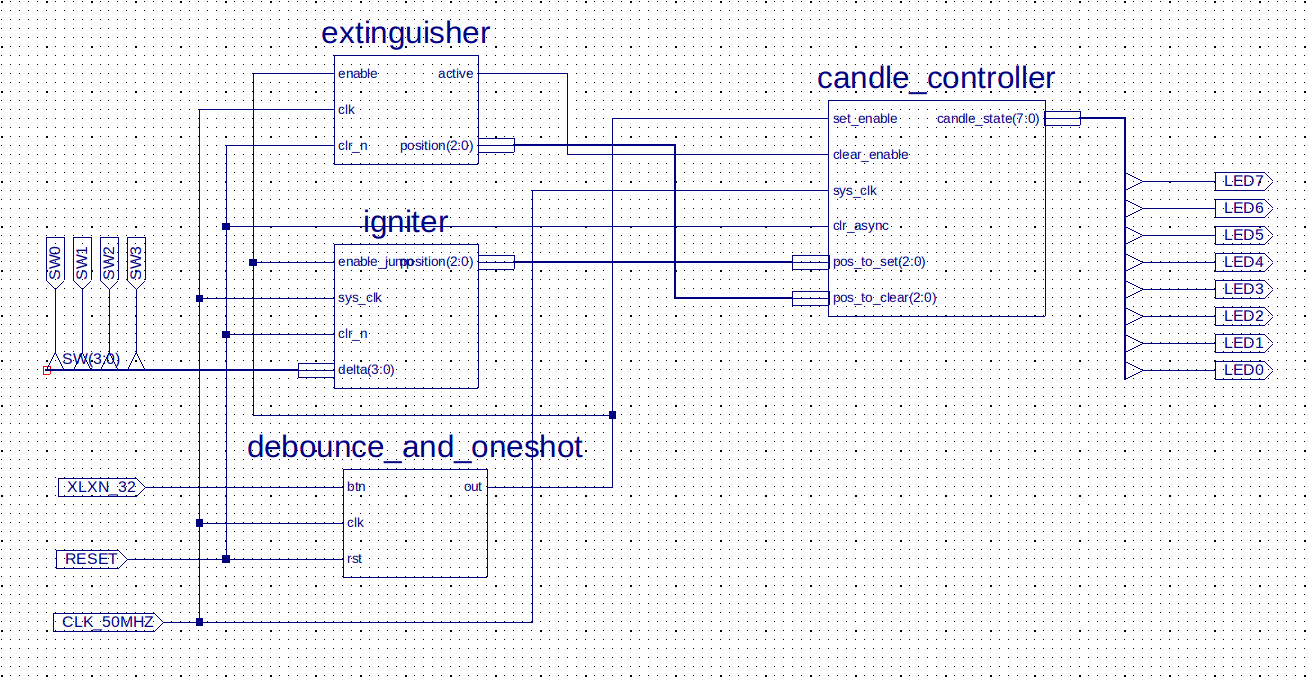
\includegraphics[width=1\textwidth]{schematic.png}
            \caption{Schematic of the Implementation of the Game} \label{fig:schematic}
        \end{center}
    \end{figure}
    \newpage

        \subsection{igniter}
        The \inlsnip{igniter} submodule allowed the player to interface with the LEDs. It accepted the 4 switches as the input, representing them as the 4 bit \inlsnip{delta} of the current position of the user. The submodule also handled BTN\_NORTH, acting as the enable.

        A testbench has been included with the project to demonstrate usage of the submodule and its effects on the position of the player in \inlsnip{igniter_tb}. A sample waveform output has been provided:

        \begin{figure}[ht]
            \begin{center}
                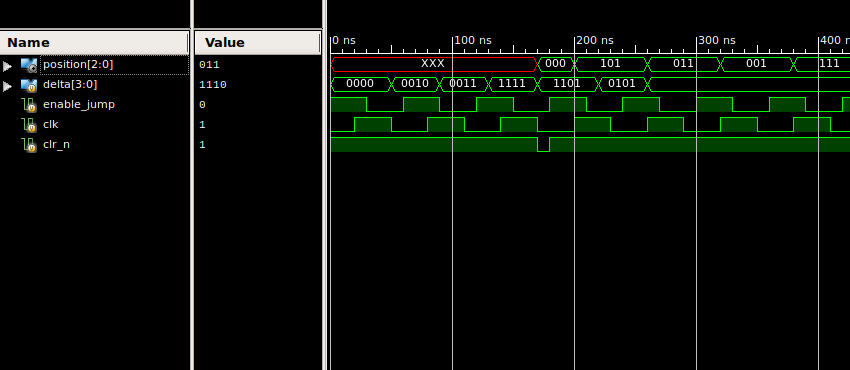
\includegraphics[width=1\textwidth]{igniter_wav.png}
                \caption{Waveform of the Testbench of igniter} \label{fig:igniter_wav}
            \end{center}
        \end{figure}
        \newpage

        \subsection{extinguisher}
        The \inlsnip{extinguisher} submodule turns the LEDs off using a pseudo-random index generator. It consists of an internal counter, running independently of the rest of the submodule on each clock cycle. The 4 bit counter iterates through all its 16 states, and outputs an active signal when the module is enabled. The active signal outputs high when the counter is less than 8 and assigns the value to the index of the LED to be turned off.

        The 50 MHz clock speed from the development board cycles through the counter very rapidly: 

         \[ 50 \ MHz=\frac{1}{50 \times 10^{6}} \ s=20 \ ns \times 16 \ states = \frac{1 \ counter \ loop}{320 \ ns} \]

        This speed allows the player to perceive the outputs of the submodule to be random.

        A testbench has been included with the project to demonstrate usage of the submodule and its effects on the position of the player in \inlsnip{extinguisher_tb}. A sample waveform output has been provided:

        \begin{figure}[ht]
            \begin{center}
                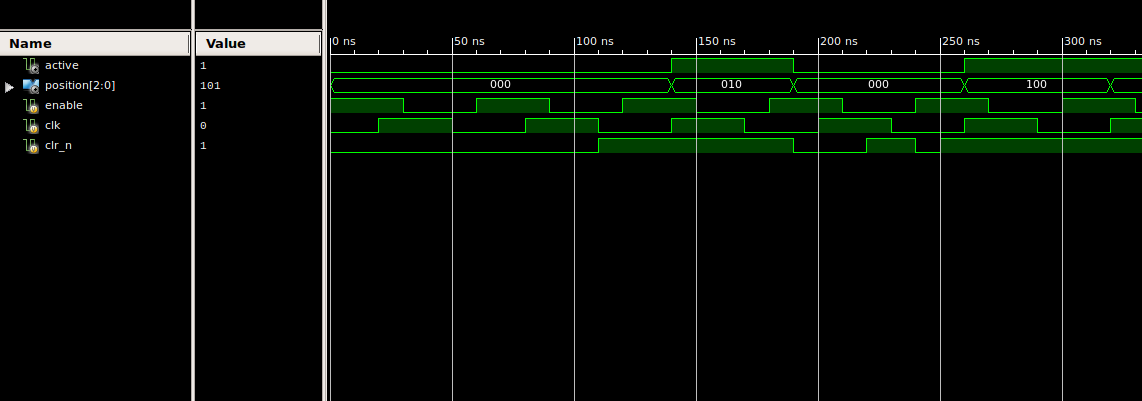
\includegraphics[width=1\textwidth]{extinguisher_wav.png}
                \caption{Waveform of the Testbench of extinguisher} \label{fig:extinguisher_wav}
            \end{center}
        \end{figure}
        \newpage

        \subsection{candle\_controller}

        The \inlsnip{candle_controller} submodule directly handles the states of the LED outputs. It utilizes the outputs from the other two submodules to determine the states of the individual LEDs.

        A testbench has been included with the project to demonstrate usage of the submodule and its effects on the position of the player in \inlsnip{candle_controller_tb}. A sample waveform output has been provided:

        \begin{figure}[ht]
            \begin{center}
                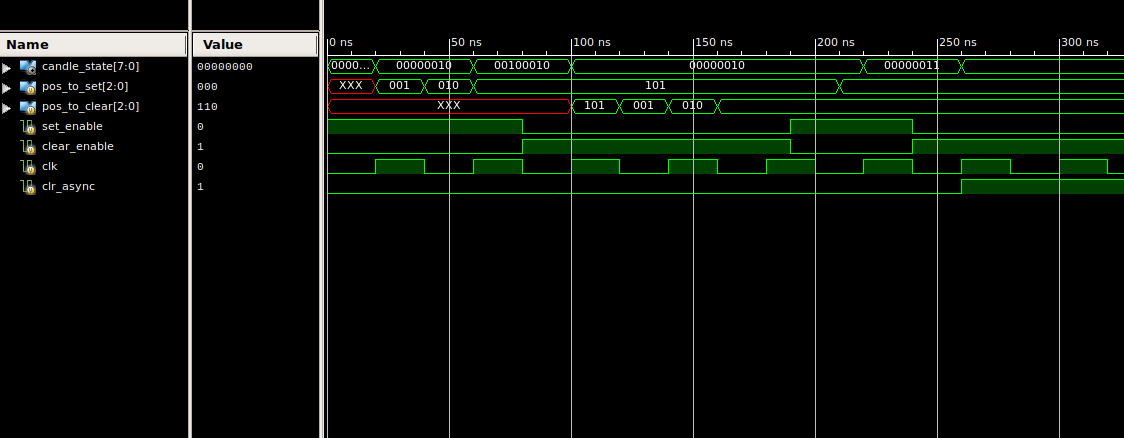
\includegraphics[width=1\textwidth]{candle_controller_wav.png}
                \caption{Waveform of the Testbench of candle\_controller} \label{fig:candle_controller_wav}
            \end{center}
        \end{figure}
        \newpage

        \subsection{Top Level Module}
        The top level module, \inlsnip{top.v}, connects all the submodules with wires. A testbench has also been included with the project to demonstrate the implementation of the game in \inlsnip{top_tb}. A sample waveform output has been provided:

        \begin{figure}[ht]
            \begin{center}
                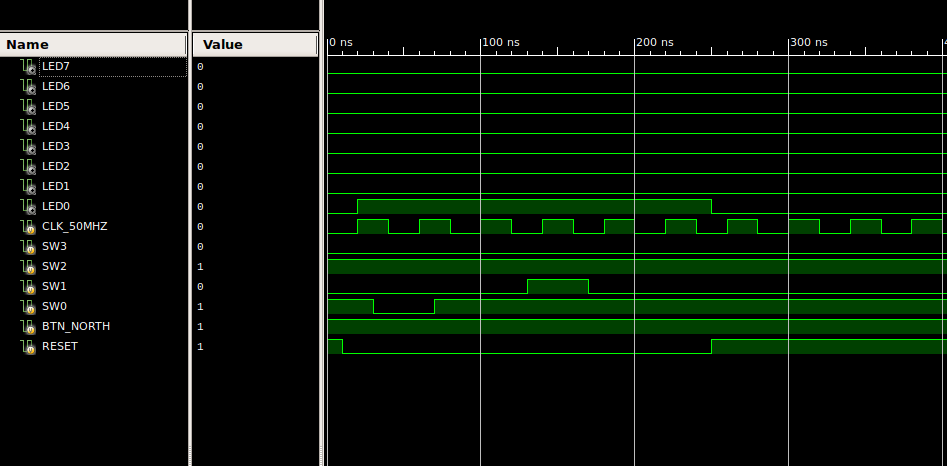
\includegraphics[width=1\textwidth]{top_wav.png}
                \caption{Waveform of the Testbench of top} \label{fig:top_wav}
            \end{center}
        \end{figure}

    \section{Troubleshooting}
    Several software and hardware issues were emphasized during the timeline of this assignment. Software glitches include the Xilinx ISE not being able to interface the development board at random times after successful synthesis. Hardware issues included the board not being able to properly process the switches as inputs in the initial stages of the assignment timeline.

    \section{Results}
    All the testbenches generated the expected outputs, and the project was successfully synthesized. The game was implemented on the board to an extent. The LEDs appear to be frozen in state when the BTN\_NORTH enable was pushed. The RESET button appear to work, but the inputs of the switches could not be validated because of the LEDs resisting to change their states.

\end{document}
